\documentclass{book}
\usepackage[english, ukrainian]{babel}
\usepackage{geometry}
\usepackage{graphicx}
\usepackage{subcaption}
\usepackage[table]{xcolor}
\usepackage[tikz]{bclogo}

\usepackage{fontspec}
\setmainfont{Arial}

\graphicspath{C:/Yola/Rozumnyky/}

\title{Історія тайнопису (криптографії).}

\begin{document}

\maketitle

\chapter*{Прості підстановковий шифр}

Уявіть, що ви сидите на уроці і хочете передати записку подружці. Але ви не
хотіли б, щоб інші діти, які б передавали цю записку чи вчителька, яка б могла
перехопити записку змогли її прочитати і зрозуміти, що там написано. Як можна
написати записку так, щоб її могли зрозуміти тільки ті кому вона призначена і
ніхто інший? Ключем для всього є "ключ". Ключ - це якісь дані, про які знають
тільки ті люди, яким дозволено читати повідомлення, які ви шлете між собою,
тобто це ваша спільний таємниця. Також треба вміти застосовувати цей ключ. Далі
ми з вами побачимо які підходи використовували люди починаючи зі стародавніх
часів, щоб зашифрувати текст, тобто перевести відкритий текст у його
зашифрований відповідник.

Перші вжитки тайнопису можна відслідкувати до більше 1500 років до н.е.
Наприклад, це робили ремісники записуючи свої рецепти, щоб зробити їх нечитними
для інших ремісників. Промотавши нитку часу далеко вперед ми бачимо, що
стародовні греки, а за ними й римляни, зокрема римський імператор Юлій Цезар послуговувалися
схожими за дією шифрами, щоб убезпечити своє листування на випадок
перехоплення. Всі ці перші шифри були підстановковими шифрами. Подивімось, що ж це
таке -- підстановковий шифр.

\subsection*{Шифр Цезаря.}

Підстановковий шифр власне підставляє. Так, все що треба зробити це вигадати
якусь схему за якою ми замість символів відкритого тексту підставлятимемо
символи шифротексту. Згаданий вище шифр Цезаря зсував усі символи на певну
відстань у абетці, ця відстань і є ключ. Наприклад, якщо ключ 1, то заміняємо
кожен символ на наступний за ним у абетці, тобто \emph{а} $\to$ \emph{б},
\emph{б} $\to$ \emph{в}, \emph{1} $\to$ \emph{2} і т.д. Останній символ абетки
заміняємо на перший, тобто йдемо по колу.

Давайте розберемось з тим як відбувається підставляння коли нам доводиться йти
по колу. Для спрощення візьмімо абетку з десяти знаків - десяти цифр. Отже,
уявімо, що нам треба зашифрувати цифру $7$ коли ключ це $5$. Для цього можна уявити
нашу абетку з цифр розміщену по колу як на годиннику. Давайте разом зробимо
п'ять кроків по колу від $7$.

\begin{figure}[hbt!]
	\centering
	\begin{subfigure}{0.17\textwidth}
		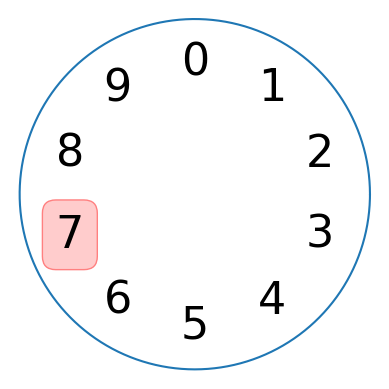
\includegraphics[width=\textwidth]{C:/Yola/Rozumnyky/crypto-history/Images/0.png}
	\end{subfigure}%
	\begin{subfigure}{0.17\textwidth}
		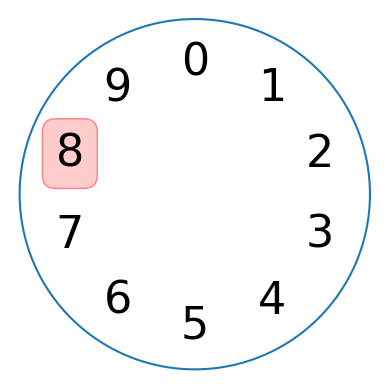
\includegraphics[width=\textwidth]{C:/Yola/Rozumnyky/crypto-history/Images/1.png}
	\end{subfigure}%
	\begin{subfigure}{0.17\textwidth}
		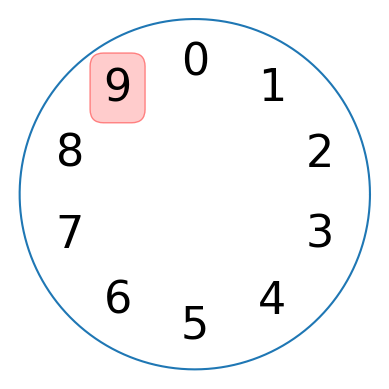
\includegraphics[width=\textwidth]{C:/Yola/Rozumnyky/crypto-history/Images/2.png}
	\end{subfigure}%
	\begin{subfigure}{0.17\textwidth}
		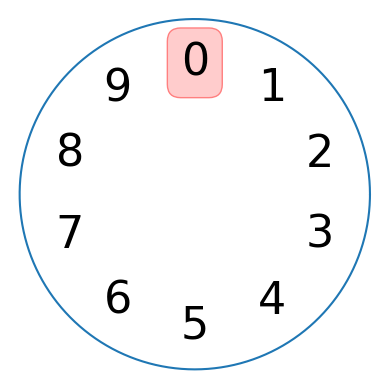
\includegraphics[width=\textwidth]{C:/Yola/Rozumnyky/crypto-history/Images/3.png}
	\end{subfigure}%
	\begin{subfigure}{0.17\textwidth}
		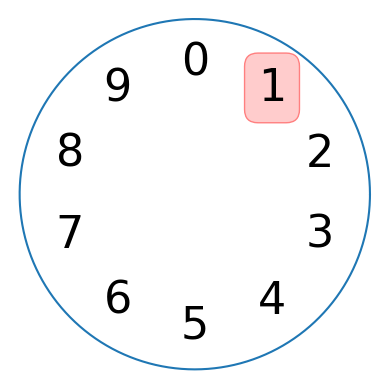
\includegraphics[width=\textwidth]{C:/Yola/Rozumnyky/crypto-history/Images/4.png}
	\end{subfigure}%
	\begin{subfigure}{0.17\textwidth}
		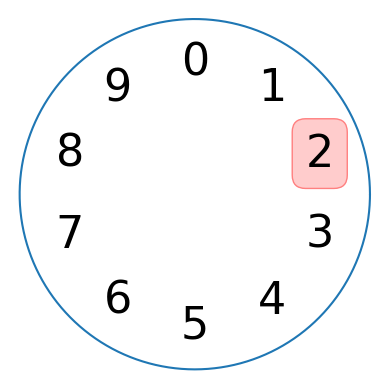
\includegraphics[width=\textwidth]{C:/Yola/Rozumnyky/crypto-history/Images/5.png}
	\end{subfigure}%
	\caption{Обчислюємо $7+5$, але ми йдемо по колу, бо найбільше доступне нам число це $9$ .}
\end{figure}

\begin{bclogo}[logo=\bcinfo, couleurBarre=orange, noborder=true, couleur=white]{Інформація}
	Таке додавання по колу, як не дивно, називається ділення за модулем. І тут
	модуль це кількість букв у абетці і записуємо ми цю дію так
	$$ 7 + 5 \equiv 2 \pmod{10} $$
	Цей вираз нам каже, що $7 + 5$ рівнозначно $2$ за модулем 10. 
\end{bclogo}

Щоб збільшити силу шифру пропуски між словами не додають в шифротекст.
Давайте спробуємо зашифрувати такий вислів:

\begin{quote}
	Єхидна, ґава, їжак ще й шиплячі плазуни бігцем форсують Янцзи.
\end{quote}

Це панграма, тобто фраза, в якій присутні всі букви абетки. Як ключ давайте
оберемо число $11$. Так буква \emph{а} перейде в \emph{і}, \emph{б} в \emph{ї} і
так далі. Ось відкритий текст і під ним шифротекст. Ви можете побачити, що
відстань між буквою відкритого тексту і її зашифрованою версією становить $11$.

\noindent
{\rowcolors{0}{blue!10}{blue!5}
\resizebox{\textwidth}{!}{
\setlength\tabcolsep{0.5pt}
\begin{tabular}{ ccccccccccccccccccccccccccccccccccccccccccccccccccc }
	Є&Х&И&Д&Н&А&Ґ&А&В&А&Ї&Ж&А&К&Щ&Е&Й&Ш&И&П&Л&Я&Ч&І&П&Л&А&З&У&Н&И&Б&І&Г&Ц&Е&М&Ф&О&Р&С&У&Ю&Т&Ь&Я&Н&Ц&З&И \\
	О&Г&С&М&Ш&І&Л&І&Й&І&У&П&І&Х&Є&Н&Ф&Е&С&Ь&Ц&И&Д&Т&Ь&Ц&І&Р&Б&Ш&С&Ї&Т&К&Ґ&Н&Ч&В&Щ&Ю&Я&Б&З&А&Ж&И&Ш&Ґ&Р&С \\
\end{tabular}
\setlength\tabcolsep{6pt}
}}

А тепер зашифруйте таке прислів'я і попросіть когось розшифрувати
отриманий вами шифротекст.

\begin{quote}
    Мудрість у ділах ліпша за мудрість у словах.
\end{quote}

Для цього скористайтесь цією таблицею підставлянь:

\begin{figure}[hbt!]
	\centering
	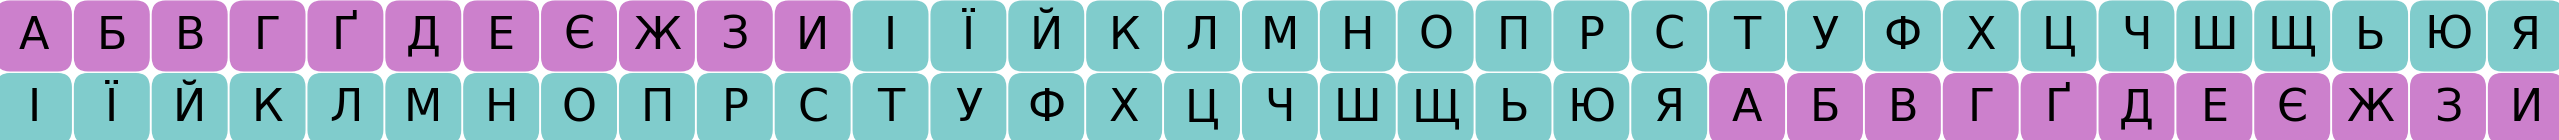
\includegraphics[width=\textwidth]{C:/Yola/Rozumnyky/crypto-history/Images/alphabet-key-11.png}
\end{figure}

Під час шифрування знаходять поточну букву з відкритого тексту в першому рядку
і замість неї підставляють букву, що розміщена прямо під нею. Зауважте, що
другий рядок утворений просуванням першого рядка по колу на $11$ позицій.

\subsection*{Зламування шифру Цезаря.}

А що як вам вдалось перехопити чиєсь повідомлення і дуже кортить дізнатись,
що ж там написано? Тоді можна спробувати зламати шифр. Спочатку подумаймо як
можна зламати шифр Цезаря. Найпростіший спосіб це перебрати всі можливі ключі,
адже їх не так багато. Порахуйте-но, скільки зсувів у абетки з 2 символів
\emph{а} і \emph{б}. Так, це $0$ і $1$. Зсув на $0$ залишає всі букви на місці,
а зсув на один міняє їх місцями. Так само як у абетки з двох символів 2 зсуви,
в абетки з 33 символів 33 різних зсуви, а отже й 33 ключі. Таку кількість ключів
можна перевірити й рукошма. От спробуйте розшифрувати такий шифротекст:

\begin{quote}
	ЄҐВИЇФФБЄҐВУРПШБЄҐВМТЇНВ
\end{quote}

Спочатку вам може здатись, що це кілька випадкових букв зібраних у рядок, але ні.
Спробуйте вгледіти якісь особливості цього тексту, можливо тут є якісь повтори?
Знайшли? Виходить, що шифротекст повторює особлвості відкритого тексту і це може
полегшити перебіг розшифрування. Отже, який ключ підійшов?

\subsection*{Шифроване послання Пилипа Орлика.}
Донині зберігся лист 1713 року від Пилипа Орлика Карлу XII. У цьому листі наш
гетьман використав складний підстановковий шифр, де букви, деякі склади і деякі
слова замінялись на дво- чи тризначні числа.


\chapter*{Багатоабеткові шифри}

\subsection*{Шифр Тритеміуса.}

Вада шифру Цезаря це те, що ключ/зсув не змінюється впродовж усього тексту і
тому його легко вирахувати. Такі шифри називають одноабетковими, їхній ключ це
відповність абетки відкритого тексту абетці шифротексту. У випадку шифру Цезаря
ключ це одна цифра, бо відповідність дуже проста "--- зсув по колу на певну
кількість символів. Цю ваду усунув Тритеміус у своєму багатоабетковому шифрі.
Він використав квадратну таблицю абеток, в якій на кожному рядку абетка була
зсунута на одну позицію далі праворуч. По суті, в таблиці записані 33 шифри
Цезаря. Усього шифр містив близько 500 замін.

\noindent{\rowcolors{3}{blue!10}{blue!5}
	\resizebox{\textwidth}{!}{
		\begin{tabular}{ cccccccccccccccccccccccccccccccccc  }
			\hline
			\multicolumn{34}{c}{Квадратна таблиця абеток} \\
			\hline
			 &А&Б&В&Г&Ґ&Д&Е&Є&Ж&З&И&І&Ї&Й&К&Л&М&Н&О&П&Р&С&Т&У&Ф&Х&Ц&Ч&Ш&Щ&Ь&Ю&Я \\
			\cellcolor[HTML]{FFFFFF}А&А&Б&В&Г&Ґ&Д&Е&Є&Ж&З&И&І&Ї&Й&К&Л&М&Н&О&П&Р&С&Т&У&Ф&Х&Ц&Ч&Ш&Щ&Ь&Ю&Я \\
			\cellcolor[HTML]{FFFFFF}Б&Б&В&Г&Ґ&Д&Е&Є&Ж&З&И&І&Ї&Й&К&Л&М&Н&О&П&Р&С&Т&У&Ф&Х&Ц&Ч&Ш&Щ&Ь&Ю&Я&А \\
			\cellcolor[HTML]{FFFFFF}В&В&Г&Ґ&Д&Е&Є&Ж&З&И&І&Ї&Й&К&Л&М&Н&О&П&Р&С&Т&У&Ф&Х&Ц&Ч&Ш&Щ&Ь&Ю&Я&А&Б \\
			\cellcolor[HTML]{FFFFFF}Г&Г&Ґ&Д&Е&Є&Ж&З&И&І&Ї&Й&К&Л&М&Н&О&П&Р&С&Т&У&Ф&Х&Ц&Ч&Ш&Щ&Ь&Ю&Я&А&Б&В \\
			\cellcolor[HTML]{FFFFFF}Ґ&Ґ&Д&Е&Є&Ж&З&И&І&Ї&Й&К&Л&М&Н&О&П&Р&С&Т&У&Ф&Х&Ц&Ч&Ш&Щ&Ь&Ю&Я&А&Б&В&Г \\
			\cellcolor[HTML]{FFFFFF}Д&Д&Е&Є&Ж&З&И&І&Ї&Й&К&Л&М&Н&О&П&Р&С&Т&У&Ф&Х&Ц&Ч&Ш&Щ&Ь&Ю&Я&А&Б&В&Г&Ґ \\
			\cellcolor[HTML]{FFFFFF}Е&Е&Є&Ж&З&И&І&Ї&Й&К&Л&М&Н&О&П&Р&С&Т&У&Ф&Х&Ц&Ч&Ш&Щ&Ь&Ю&Я&А&Б&В&Г&Ґ&Д \\
			\cellcolor[HTML]{FFFFFF}Є&Є&Ж&З&И&І&Ї&Й&К&Л&М&Н&О&П&Р&С&Т&У&Ф&Х&Ц&Ч&Ш&Щ&Ь&Ю&Я&А&Б&В&Г&Ґ&Д&Е \\
			\cellcolor[HTML]{FFFFFF}Ж&Ж&З&И&І&Ї&Й&К&Л&М&Н&О&П&Р&С&Т&У&Ф&Х&Ц&Ч&Ш&Щ&Ь&Ю&Я&А&Б&В&Г&Ґ&Д&Е&Є \\
			\cellcolor[HTML]{FFFFFF}З&З&И&І&Ї&Й&К&Л&М&Н&О&П&Р&С&Т&У&Ф&Х&Ц&Ч&Ш&Щ&Ь&Ю&Я&А&Б&В&Г&Ґ&Д&Е&Є&Ж \\
			\cellcolor[HTML]{FFFFFF}И&И&І&Ї&Й&К&Л&М&Н&О&П&Р&С&Т&У&Ф&Х&Ц&Ч&Ш&Щ&Ь&Ю&Я&А&Б&В&Г&Ґ&Д&Е&Є&Ж&З \\
			\cellcolor[HTML]{FFFFFF}І&І&Ї&Й&К&Л&М&Н&О&П&Р&С&Т&У&Ф&Х&Ц&Ч&Ш&Щ&Ь&Ю&Я&А&Б&В&Г&Ґ&Д&Е&Є&Ж&З&И \\
			\cellcolor[HTML]{FFFFFF}Ї&Ї&Й&К&Л&М&Н&О&П&Р&С&Т&У&Ф&Х&Ц&Ч&Ш&Щ&Ь&Ю&Я&А&Б&В&Г&Ґ&Д&Е&Є&Ж&З&И&І \\
			\cellcolor[HTML]{FFFFFF}Й&Й&К&Л&М&Н&О&П&Р&С&Т&У&Ф&Х&Ц&Ч&Ш&Щ&Ь&Ю&Я&А&Б&В&Г&Ґ&Д&Е&Є&Ж&З&И&І&Ї \\
			\cellcolor[HTML]{FFFFFF}К&К&Л&М&Н&О&П&Р&С&Т&У&Ф&Х&Ц&Ч&Ш&Щ&Ь&Ю&Я&А&Б&В&Г&Ґ&Д&Е&Є&Ж&З&И&І&Ї&Й \\
			\cellcolor[HTML]{FFFFFF}Л&Л&М&Н&О&П&Р&С&Т&У&Ф&Х&Ц&Ч&Ш&Щ&Ь&Ю&Я&А&Б&В&Г&Ґ&Д&Е&Є&Ж&З&И&І&Ї&Й&К \\
			\cellcolor[HTML]{FFFFFF}М&М&Н&О&П&Р&С&Т&У&Ф&Х&Ц&Ч&Ш&Щ&Ь&Ю&Я&А&Б&В&Г&Ґ&Д&Е&Є&Ж&З&И&І&Ї&Й&К&Л \\
			\cellcolor[HTML]{FFFFFF}Н&Н&О&П&Р&С&Т&У&Ф&Х&Ц&Ч&Ш&Щ&Ь&Ю&Я&А&Б&В&Г&Ґ&Д&Е&Є&Ж&З&И&І&Ї&Й&К&Л&М \\
			\cellcolor[HTML]{FFFFFF}О&О&П&Р&С&Т&У&Ф&Х&Ц&Ч&Ш&Щ&Ь&Ю&Я&А&Б&В&Г&Ґ&Д&Е&Є&Ж&З&И&І&Ї&Й&К&Л&М&Н \\
			\cellcolor[HTML]{FFFFFF}П&П&Р&С&Т&У&Ф&Х&Ц&Ч&Ш&Щ&Ь&Ю&Я&А&Б&В&Г&Ґ&Д&Е&Є&Ж&З&И&І&Ї&Й&К&Л&М&Н&О \\
			\cellcolor[HTML]{FFFFFF}Р&Р&С&Т&У&Ф&Х&Ц&Ч&Ш&Щ&Ь&Ю&Я&А&Б&В&Г&Ґ&Д&Е&Є&Ж&З&И&І&Ї&Й&К&Л&М&Н&О&П \\
			\cellcolor[HTML]{FFFFFF}С&С&Т&У&Ф&Х&Ц&Ч&Ш&Щ&Ь&Ю&Я&А&Б&В&Г&Ґ&Д&Е&Є&Ж&З&И&І&Ї&Й&К&Л&М&Н&О&П&Р \\
			\cellcolor[HTML]{FFFFFF}Т&Т&У&Ф&Х&Ц&Ч&Ш&Щ&Ь&Ю&Я&А&Б&В&Г&Ґ&Д&Е&Є&Ж&З&И&І&Ї&Й&К&Л&М&Н&О&П&Р&С \\
			\cellcolor[HTML]{FFFFFF}У&У&Ф&Х&Ц&Ч&Ш&Щ&Ь&Ю&Я&А&Б&В&Г&Ґ&Д&Е&Є&Ж&З&И&І&Ї&Й&К&Л&М&Н&О&П&Р&С&Т \\
			\cellcolor[HTML]{FFFFFF}Ф&Ф&Х&Ц&Ч&Ш&Щ&Ь&Ю&Я&А&Б&В&Г&Ґ&Д&Е&Є&Ж&З&И&І&Ї&Й&К&Л&М&Н&О&П&Р&С&Т&У \\
			\cellcolor[HTML]{FFFFFF}Х&Х&Ц&Ч&Ш&Щ&Ь&Ю&Я&А&Б&В&Г&Ґ&Д&Е&Є&Ж&З&И&І&Ї&Й&К&Л&М&Н&О&П&Р&С&Т&У&Ф \\
			\cellcolor[HTML]{FFFFFF}Ц&Ц&Ч&Ш&Щ&Ь&Ю&Я&А&Б&В&Г&Ґ&Д&Е&Є&Ж&З&И&І&Ї&Й&К&Л&М&Н&О&П&Р&С&Т&У&Ф&Х \\
			\cellcolor[HTML]{FFFFFF}Ч&Ч&Ш&Щ&Ь&Ю&Я&А&Б&В&Г&Ґ&Д&Е&Є&Ж&З&И&І&Ї&Й&К&Л&М&Н&О&П&Р&С&Т&У&Ф&Х&Ц \\
			\cellcolor[HTML]{FFFFFF}Ш&Ш&Щ&Ь&Ю&Я&А&Б&В&Г&Ґ&Д&Е&Є&Ж&З&И&І&Ї&Й&К&Л&М&Н&О&П&Р&С&Т&У&Ф&Х&Ц&Ч \\
			\cellcolor[HTML]{FFFFFF}Щ&Щ&Ь&Ю&Я&А&Б&В&Г&Ґ&Д&Е&Є&Ж&З&И&І&Ї&Й&К&Л&М&Н&О&П&Р&С&Т&У&Ф&Х&Ц&Ч&Ш \\
			\cellcolor[HTML]{FFFFFF}Ь&Ь&Ю&Я&А&Б&В&Г&Ґ&Д&Е&Є&Ж&З&И&І&Ї&Й&К&Л&М&Н&О&П&Р&С&Т&У&Ф&Х&Ц&Ч&Ш&Щ \\
			\cellcolor[HTML]{FFFFFF}Ю&Ю&Я&А&Б&В&Г&Ґ&Д&Е&Є&Ж&З&И&І&Ї&Й&К&Л&М&Н&О&П&Р&С&Т&У&Ф&Х&Ц&Ч&Ш&Щ&Ь \\
			\cellcolor[HTML]{FFFFFF}Я&Я&А&Б&В&Г&Ґ&Д&Е&Є&Ж&З&И&І&Ї&Й&К&Л&М&Н&О&П&Р&С&Т&У&Ф&Х&Ц&Ч&Ш&Щ&Ь&Ю \\
			\hline
		\end{tabular}
	}

Зазвичай для шифрування букви відкритого тексту одну за одною знаходять у лівому
заголовковому стовбці і заміняють на букву з відповідного стовбця в тому ж
рядку. Номер стовпця це просто номер букви у відкритому тексті. Звісно, ми тут
також ходимо по колу, тобто, для позиції \#1 беремо стовбець \#1, для позиції \#33
стовбець \#33 і далі по колу "--- для позиції \#34 використовуємо стовбець \#1,
і т.д. Таким чином, слово \emph{СМАКОЛИК} кодуємо в \emph{СНВНТРМС}.

Спробуйте самі зрозуміти як розшифровувати текст і розшифруйте шифротекст
\emph{МЇЧССУБЄ}.

Обернену дію (розшифрування) виконуємо так "--- знов лівий заголовковий стовбець
це букви відкритого тексту, а ми йдемо по шифротексту переходячи до наступного
стовбця з кожною наступною буквою і шукаємо цю букву в цьому стовбці, знаходячи
рядок заголовкова буква якого і є шуканою буквою відкритого тексту.

\subsection*{Шифр Віженера.}

Цікаво, що шифр Тритеміуса не має ключа. А це означає, що якщо супротивник перехопив
повідомлення і знає, що ми використали шифр Тритеміуса, то він з легкістю його
розшифрує. Тут нам допоможе придумка італійського криптографа Джованні Баттіста
Белласи, яку в 19-му сторіччі помилково приписали Блезу де Віженеру, звідки й
сучасна назва.

Придумка дуже проста, обрати ключове слово і утворити ключ повторюючи
ключове слово допоки ключ не уоднаковиться завдовжки з відкритим
текстом. Наприклад, для відкритого тексту \emph{справа майстра величає} і
ключового слова \emph{таємниця} ключ утворюємо так:

\noindent
	\setlength\tabcolsep{0.5pt}
	\begin{tabular}{ lcccccccccccccccccccc }
		Відкритий текст&С&П&Р&А&В&А&М&А&Й&С&Т&Р&А&В&Е&Л&И&Ч&А&Є \\
		Ключ&Т&А&Є&М&Н&И&Ц&Я&Т&А&Є&М&Н&И&Ц&Я&Т&А&Є&М \\
	\end{tabular}
	\setlength\tabcolsep{6pt}

І тепер, якщо в шифрі Тритеміуса ми дивились на стовбці в наперед визначеному
порядку, кожен раз пересуваючись на одну букву праворуч, то тепер ми стрибаємо
по стовбцях відповідно до букв у ключі. Наприклад, спершу ми подивимось у
стовбець \#22, бо в заголовковому рядку в позиції \#22 стоїть буква \emph{Т}.
У висліді шифрування отримуємо \emph{ИПЧМПИЗЯВСЩГНЇЯКЯЧЄУ}.

Спробуйте власноруч розшифрувати \emph{КТХҐКАЄЗБВЯДВЮУТҐЬЗЧПЦГТГОЖТЯЗЄЗ} з
ключем утвореним з того самого слова. Тут ви в шифротексті вже не побачите
тих повторів, що їх можна побачити у відкритому тексті.

Цей шифр винайдений у 1553 році пробув незламним близько трьох століть, допоки
його не зламав Чарлз Бебідж.

\subsection*{Одноразовий блокнот. Незламний?}

Техніка одноразового блокноту дозволяє шифрування, яке неможливо розшифрувати.
Але є одне але, ця техніка вимагає ключа щонайменше такого ж завдовжки як і саме
повідомлення. Тоді, щоб отирмати шифротекст, можна одну за одною додавати між
собою букви відкритого тексту і ключа. Давайте зашифруємо слово \emph{мрія}
ключем \emph{гарт}. Спочатку перенумеруємо букви абетки.


\noindent{
	\resizebox{\textwidth}{!}{
		\begin{tabular}{ ccccccccccccccccccccccccccccccccc  }
			\hline
			1&2&3&4&5&6&7&8&9&10&11&12&13&14&15&16&17&18&19&20&21&22&23&24&25&26&27&28&29&30&31&32&33 \\
			А&Б&В&Г&Ґ&Д&Е&Є&Ж&З&И&І&Ї&Й&К&Л&М&Н&О&П&Р&С&Т&У&Ф&Х&Ц&Ч&Ш&Щ&Ь&Ю&Я \\
			\hline
		\end{tabular}
	}

Отже, додаємо, але пам'ятаємо, що ми додаємо по колу (за модулем), тобто коли
ми вибігаємо за межі абетки, ми повертаємось на її початок.

\noindent
\begin{tabular}{ ccccccccccccc  }
	\hline
	М&+&Г&=&17&+&4&=&21&&&=&Р\\
	Р&+&А&=&21&+&1&=&22&&&=&С\\
	І&+&Р&=&13&+&21&=&33&+&1&=&А\\
	Я&+&Т&=&33&+&23&=&33&+&23&=&Т\\
	\hline
\end{tabular}

Як я вже згадував, вада цього шифру це необхідність мати ключ завдовжки
щонайменше з повідомлення. Ба більше, якщо постійно використовувати один і той
самий ключ, то це дасть перехопникам шанс розгадати цей ключ. Але якже бути,
це ж незручно кожен раз передавати великий ключ, адже якби ми могли надійно
передавати великі ключи, то ми так само могли б передавати й наші повідомлення
не шифруючи їх. А що, якщо в якості ключа взяти текст з якоїсь книжки? Це
може спрацювати, адже можна домовитись про книгу і як в ній знаходити ключ для
кожного наступного повідомлення.

Поговорімо про \emph{незламність} цього шифру. Цей шифр дійсно може бути
незламним, але для цього мають виконуватись кілька умов на ключ:
\begin{enumerate}
	\item Ключ має бути не коротшим ніж текст.
	\item Ключ має складатись з випадково обраних букв.
	\item Ключ можна використовувати лише один раз.
	\item Ключ має триматись у таємниці.
\end{enumerate}

На цьому я завершу огляд тайнопису. Розглянуті шифри ви можете використовувати
маючи під рукою лише папір і ручку, але якщо вам треба буде зашифрувати справді
довге повідомлення, то без якоїсь автоматизмції, на штиб написання комп'ютерної
програми, вам не обійтись.

\subsection*{Відповіді.}

\begin{enumerate}
\item Шифротекст "--- \emph{ЧБМЮТЯАЖБМТЦІГЦТЬЕІРІЧБМЮТЯАЖБЯЦЩЙІГ.}
\item Зсув "--- $3$, текст "--- \emph{Два життя, два сонця, два крила.}
\item Текст "--- \emph{міхоноша.}
\item Текст "--- \emph{Хтось у Київ, хтось у Львів, ми – у Кобеляки!}
\end{enumerate}

\end{document}
